\section{三类积分之间的关系}
\label{sec:multivariable-boundary-relations}

一元微积分基本定理说，若$f$在$[a,b]$上连续可微，则导数$f'$在区间上的积分等于$f(b)-f(a)$：区间内部各点的变化率累计起来，只剩下两个端点上的函数值。
区间的边界就是这两个端点，所以$f(b)-f(a)$也可以读成带符号的边界求和：右端点记正号，左端点记负号。
路径积分基本定理（式~\eqref{eq:analysis-line-integral-gradient}）把同样的关系搬到路径上：梯度场沿路径的积分，等于势函数在终点与起点的值之差。

本节把这种“内部导数的累计等于边界上的累计”的关系推广到平面区域、空间区域和曲面。
三种推广共用一个思路。先把对象切成许多小块；在每个小块上，某个导数乘小块的大小，近似等于向量场沿小块边界的累计。
相邻两块的公共边界被两块各算一次，两次的方向相反，相加后抵消，最后只剩下整个对象的外边界。
按边界的类型，本节回答三个问题：平面区域上的积分何时等于边界路径积分，这是Green公式；空间区域上的积分何时等于边界曲面积分，这是Gauss公式；曲面上的积分何时等于曲面边界的路径积分，这是Stokes公式。

这些公式中的被积对象不能互换。沿边界的环流累计向量场的切向分量，对应的内部量是旋度，它衡量场绕一点旋转的强度；
穿过边界的通量累计向量场的法向分量，对应的内部量是散度，它衡量场从一点向外发散的强度。

为此，本节先定义这两种导数以及Laplace算子，并说明它们的物理含义；再规定边界的方向；最后给出各公式的条件、推导和例子。
所有区域积分以及路径、曲面的参数积分均采用勒贝格积分。经典公式的组织参考向量微积分教材\scite{math-openstax-calculus3}。

\subsection{积分公式中的微分算子}

定义~\ref{def:multivariable-gradient}把标量函数的各个一阶偏导数排成梯度。现在考虑开集$U$上的向量场$\bm F$，不妨把它想成流体的速度场：$\bm F(\bm x)$是流体在位置$\bm x$处的速度。
对这样的场，有两个自然的局部问题：在一点附近，流体是净流出还是净流入；流体是否绕这一点打转。
两个问题的答案都由$\bm F$各分量的一阶偏导数决定，但用到的偏导数组合不同。
回答前一个问题的是散度，回答后一个问题的是旋度，二者都以向量场为输入；随后的Laplace算子以标量函数为输入，比较函数在一点的值与周围平均值的差别。

\subsubsection{散度}

\paragraph{小立方体的净流出}

设$\bm F=(F_1,F_2,F_3)^\top$是三维流体的速度场。第~\ref{sec:analysis-surface-integration}节定义的通量只取速度的法向分量，原因如下。
在很短的时间$\Delta t$内，穿过面积为$\Delta S$、单位法向为$\bm n$的一小片曲面的流体，占据一个底面积为$\Delta S$、高约为$(\bm F^\top\bm n)\Delta t$的斜柱；所以单位时间穿过这一小片的流体体积约为$(\bm F^\top\bm n)\Delta S$，速度的切向分量只让流体沿曲面滑动，不贡献穿过量。
现在以点$\bm a$为中心取边长为$h$的小立方体，各面与坐标平面平行，估计单位时间从它流出的净体积。

先看与$x$轴垂直的两张面。右面$x=a_1+h/2$的外法向是$\bm e_1$，场在这张面上的法向分量是$F_1$；用面中心的值代表整张面，流出量约为$F_1(\bm a+\tfrac h2\bm e_1)h^2$。
左面$x=a_1-h/2$的外法向是$-\bm e_1$，流出量约为$-F_1(\bm a-\tfrac h2\bm e_1)h^2$；$F_1>0$时这个量为负，表示沿$x$正方向的流动在左面是流入。两面合计为
\[
 \Bigl[F_1\bigl(\bm a+\tfrac h2\bm e_1\bigr)-F_1\bigl(\bm a-\tfrac h2\bm e_1\bigr)\Bigr]h^2
 \approx \partial_1F_1(\bm a)\,h\cdot h^2,
\]
这里用偏导数乘距离$h$近似了$F_1$在两张面中心之间的差。
若$F_1$沿$x$方向增大，从右面流出的比从左面流入的多，这对面贡献正的净流出；若$F_1$沿$x$方向不变，流入与流出恰好相等。

另外两对面同样分别给出约$\partial_2F_2(\bm a)h^3$和$\partial_3F_3(\bm a)h^3$。六张面合计后除以体积$h^3$，得到
\[
 \frac{\text{小立方体的净流出}}{\text{小立方体的体积}}
 \approx\partial_1F_1(\bm a)+\partial_2F_2(\bm a)+\partial_3F_3(\bm a).
\]
这里只做了一阶近似。在Gauss公式（定理~\ref{thm:analysis-divergence-theorem}）之后将证明，当$\bm F$连续可微且$h\to0$时，左侧确实收敛到右侧。右侧的偏导数之和称为散度。
\begin{definition}[散度]
\label{def:multivariable-divergence}
设$U\subseteq\mathbb R^d$为开集，$\bm F=(F_1,\ldots,F_d)^\top:U\to\mathbb R^d$的各分量一阶偏导数存在。
$\bm F$的\term{散度}（divergence）是标量函数
\[
 \operatorname{div}\bm F
 =\nabla\mathbin{\cdot}\bm F
 =\sum_{j=1}^d\partial_jF_j.
\]
\end{definition}

\paragraph{源的强度}

按小立方体上的推导，散度是单位体积的净流出率，可以理解为一点处“源”的强度。
$\operatorname{div}\bm F(\bm a)>0$表示$\bm a$附近像有一个源，流体在这里产生并向外流走；$\operatorname{div}\bm F(\bm a)<0$表示这里像一个汇，流入的多于流出的；散度为零表示流入与流出平衡。
若流体不可压缩，内部又没有注入或抽出流体的源和汇，则每个小体积的流入量都等于流出量，速度场的散度处处为零。

下面三个场分别对应均匀膨胀、绕轴转动和整体平移，可以用来检验这一解释。
\begin{example}[径向场、旋转场与常场的散度]
三维径向场$\bm F(x,y,z)=(x,y,z)^\top$满足$\partial_xF_1=\partial_yF_2=\partial_zF_3=1$，所以$\operatorname{div}\bm F=1+1+1=3$：流体从各处均匀地向外膨胀，每单位体积每单位时间多出$3$个单位体积的流体。

旋转场$\bm G(x,y,z)=(-y,x,0)^\top$的第一分量不含$x$，第二分量不含$y$，第三分量为零，所以$\operatorname{div}\bm G=0+0+0=0$：流体绕$z$轴转动，任何小立方体流入多少就流出多少。

常场$\bm H=(1,0,0)^\top$的各分量都是常数，散度同样为$0$：流体整体平移，每个小立方体从左面流入的量都从右面流出。
\end{example}
旋转场和常场都不是零场，散度却都为零。可见散度为零只表示局部净流出率为零，并不表示向量场为零。

二维场$(P,Q)^\top$的散度相应为$P_x+Q_y$，它是小正方形四条边上的净流出除以面积所得的极限；定理~\ref{thm:multivariable-planar-flux}的平面通量公式使用这一标量函数。

\subsubsection{旋度}

\paragraph{小正方形上的环流}

净流出不能描述绕一点旋转的运动。旋转场$\bm G=(-y,x,0)^\top$的散度为零，但在水平平面内沿以$z$轴上一点为圆心的圆周逆时针走一圈，场始终与行进方向相同，环流不为零。
为了度量一点附近的旋转，先在平面上计算小正方形边界的环流。设平面场为$(P,Q)^\top$，以$\bm a$为中心取边长为$h$的正方形，沿逆时针方向走一圈。

下边从左向右，切向分量是$P$，贡献约$P(\bm a-\tfrac h2\bm e_2)h$；上边从右向左，贡献约$-P(\bm a+\tfrac h2\bm e_2)h$；两者合计约$-\partial_yP(\bm a)h^2$。
右边从下向上，贡献约$Q(\bm a+\tfrac h2\bm e_1)h$；左边从上向下，贡献约$-Q(\bm a-\tfrac h2\bm e_1)h$；两者合计约$\partial_xQ(\bm a)h^2$。四边相加后除以面积$h^2$，得到
\[
 \frac{\text{小正方形边界的逆时针环流}}{\text{小正方形的面积}}
 \approx\partial_xQ(\bm a)-\partial_yP(\bm a).
\]
两项的符号可以这样理解。若$Q$沿$x$方向增大，右边向上的流速比左边大，这一对边推动逆时针转动；若$P$沿$y$方向增大，上边向右的流速比下边大，这一对边推动顺时针转动，所以$\partial_yP$带负号。

在三维空间中，小正方形可以放在分别垂直于三个坐标轴的平面里，行进方向都取从相应坐标轴正方向看的逆时针。
垂直于$z$轴时，平面坐标是$(x,y)$，$(F_1,F_2)$相当于$(P,Q)$，同样的计算给出$\partial_xF_2-\partial_yF_1$；
垂直于$x$轴时，平面坐标的次序是$(y,z)$，$(F_2,F_3)$相当于$(P,Q)$，得到$\partial_yF_3-\partial_zF_2$；
垂直于$y$轴时，平面坐标的次序是$(z,x)$，$(F_3,F_1)$相当于$(P,Q)$，得到$\partial_zF_1-\partial_xF_3$。
这样选取坐标次序，是因为$\bm e_2\times\bm e_3=\bm e_1$、$\bm e_3\times\bm e_1=\bm e_2$：从坐标轴正方向看，第一个平面坐标轴逆时针转过直角得到第二个。
把这三个环流率按$x,y,z$轴的次序排成一个向量，就得到旋度。
\begin{definition}[旋度]
\label{def:multivariable-curl}
设$U\subseteq\mathbb R^3$为开集，$\bm F=(F_1,F_2,F_3)^\top:U\to\mathbb R^3$的各分量一阶偏导数存在。
$\bm F$的\term{旋度}（curl）是向量场
\[
 \operatorname{curl}\bm F=\nabla\times\bm F
 =\begin{pmatrix}
   \partial_yF_3-\partial_zF_2\\
   \partial_zF_1-\partial_xF_3\\
   \partial_xF_2-\partial_yF_1
  \end{pmatrix}.
\]
\end{definition}

\paragraph{旋转的轴与强度}

坐标平面上的三个计算可以推广到任意方向。设$\bm F$连续可微，$\bm n$是单位向量；在过点$\bm a$且垂直于$\bm n$的平面内，取以$\bm a$为中心的小正方形或小圆周，从$\bm n$的箭头一侧看按逆时针行进。
尺寸趋于零时，环流除以所围面积的极限等于$(\operatorname{curl}\bm F)(\bm a)^\top\bm n$。$\bm n$为坐标轴方向时，这就是上面的计算；一般方向的证明放在Stokes公式之后。

由Cauchy--Schwarz不等式，$(\operatorname{curl}\bm F)^\top\bm n\leq\lVert\operatorname{curl}\bm F\rVert_2$；旋度不为零时，等号当且仅当$\bm n$与旋度同向时成立。
所以旋度的方向是局部旋转最强的转轴，其长度是旋转的强度；转向由右手定则确定：右手大拇指沿旋度方向，其余四指弯曲的方向就是转向。

一个物理图像是放进流水中的小桨轮。让桨轮的转轴沿$\bm n$，水流沿轮缘推动各个叶片；桨轮是否转动、往哪边转，取决于沿轮缘的环流，也就是$(\operatorname{curl}\bm F)^\top\bm n$的符号；转轴与旋度平行时转得最快。
这一图像帮助理解定义，但不代替上面的计算。

先用整体转动和径向膨胀检验这一图像。
\begin{example}[刚体旋转与径向膨胀的旋度]
\label{ex:analysis-rigid-rotation-curl}
整体以角速度$\omega$绕$z$轴旋转的流体，速度场为$\bm F=\omega(-y,x,0)^\top$。代入定义，前两个分量$\partial_yF_3-\partial_zF_2$与$\partial_zF_1-\partial_xF_3$都为零，第三个分量为$\partial_x(\omega x)-\partial_y(-\omega y)=2\omega$，所以$\nabla\times\bm F=(0,0,2\omega)^\top$。
特别地，$\omega=1/2$时$\bm F=(-y/2,x/2,0)^\top$，旋度为$(0,0,1)^\top$。

径向场$(x,y,z)^\top$的第$i$个分量只依赖第$i$个坐标，旋度定义中的每个交叉偏导数都为零，所以旋度为零：流体只向外膨胀而不打转。
\end{example}
刚体旋转的旋度沿转轴，长度是角速度的两倍，与桨轮图像一致。不过，旋度与流线是否弯曲并不是一回事，下面两个场从相反的方向说明这一点。
\begin{example}[剪切流与涡旋场]
剪切流$\bm F=(y,0,0)^\top$的流线都是水平直线。它的偏导数中只有$\partial_yF_1=1$不为零，所以$\nabla\times\bm F=(0,0,-1)^\top$。
物理上，上方的水比下方的水向右流得快，桨轮的上缘被推得更多，从$z$轴正方向看桨轮顺时针转动，与第三分量为负一致。

再看平面上沿同心圆流动的场。设流体在每个以原点为圆心的圆周上逆时针流动，半径为$r$的圆周上速率为$s(r)>0$，其中$s$可微，即
\[
 (P,Q)^\top=g(r)\,(-y,x)^\top,\qquad g(r)=\frac{s(r)}r,\quad r=\sqrt{x^2+y^2}>0.
\]
由$\partial_xr=x/r$、$\partial_yr=y/r$，有$Q_x=g(r)+g'(r)x^2/r$、$P_y=-g(r)-g'(r)y^2/r$，所以
\[
 Q_x-P_y=2g(r)+rg'(r)=\frac{s(r)}r+s'(r).
\]
第一项$s(r)/r$来自流线的弯曲，第二项$s'(r)$来自不同半径上流速的差别。刚体旋转$s(r)=\omega r$时两项都等于$\omega$，合计$2\omega$，与前例一致。
第~\ref{sec:multivariable-potential-path-independence}节穿孔平面上的涡旋场$(-y,x)^\top/(x^2+y^2)$对应$s(r)=1/r$，两项分别为$1/r^2$与$-1/r^2$，所以在原点以外$Q_x-P_y=0$。
\end{example}
剪切流的流线是直线，旋度却不为零；涡旋场的流线弯曲，在原点以外旋度却为零。后者的原因是：流线弯曲带来的逆时针倾向，恰好被外侧流速较慢带来的顺时针倾向抵消，所以放在原点以外的小桨轮不转。

对二维场$(P,Q)^\top$，平面内需要的是标量$Q_x-P_y$。
把二维场补上为零的第三分量，写成三维场$(P,Q,0)^\top$后，这一标量正是旋度的第三分量，也就是旋度在向上法向$\bm e_3$上的分量。
符号$\nabla\mathbin\cdot$和$\nabla\times$表示这里定义的偏导数组合，不是两个普通数值向量的内积或叉积。


图~\ref{fig:analysis-process-divergence-circulation-fields}在同一个单位圆周上分别观察净流出与切向环流，比较两种微分算子所记录的信息。
\begin{figure*}[!htbp]
 \centering
 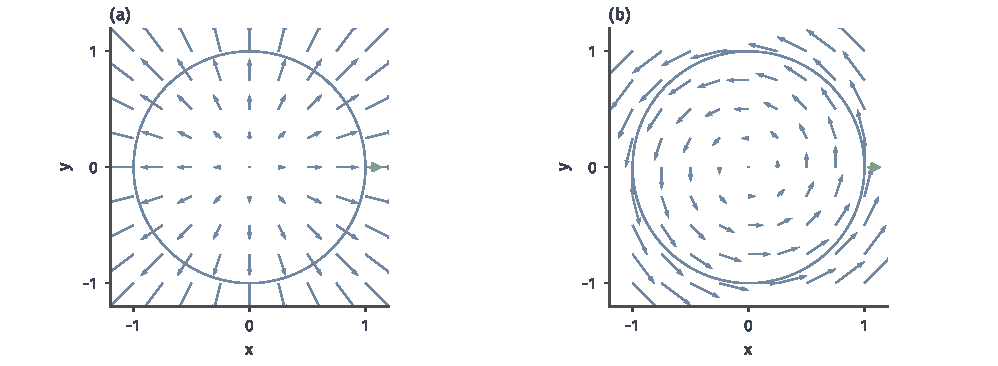
\includegraphics[width=169.0mm]{figures/01-mathematical-preliminaries-upper/01-mathematical-language-combinatorics-analysis-optimization/matplotlib/chapter3-concept-processes/divergence-circulation-fields.pdf}
 \caption{(a) 径向场$(x,y)^\top$的二维散度为$2$、旋转率$Q_x-P_y=0$，圆周外向通量为$2\pi$、环流为零。(b) 旋转场$(-y,x)^\top$的散度为零、旋转率为$2$，通量为零、环流为$2\pi$。绿箭头仅标记外法向；蓝色场箭头按相同常数缩放。零散度不等于零场，也不等于零环流。}
 \label{fig:analysis-process-divergence-circulation-fields}
\end{figure*}

\subsubsection{Laplace算子}

标量函数的梯度是向量场，因此可以对它继续取散度，把各坐标方向的二阶变化相加。
这一复合运算出现在多元分部积分中，也出现在描述热传导和扩散的方程中；它的输入与输出都是标量函数。
\begin{definition}[Laplace算子]
\label{def:multivariable-laplacian}
对开集$U\subseteq\mathbb R^d$上的二阶连续可微标量函数$v$，定义\term{Laplace算子}（Laplacian）为
\[
 \Delta v=\operatorname{div}(\nabla v)
 =\sum_{j=1}^d\partial_j^2v.
\]
\end{definition}
梯度把标量函数变为向量场，散度再把向量场变为标量函数，所以$\Delta v$仍是标量函数；它与输入、输出都是向量场的旋度属于不同类型的运算。

\paragraph{与邻域平均值的差}

一元情形中，$v''(a)>0$表示函数在$a$附近向上弯，$v(a)$低于两侧邻点的平均值。多元情形可以做同样的比较。
在$\bm a$的每个坐标方向上各取前后两个邻点$\bm a\pm h\bm e_j$，沿该坐标作二阶Taylor展开：
\[
 v(\bm a+h\bm e_j)+v(\bm a-h\bm e_j)-2v(\bm a)=h^2\partial_j^2v(\bm a)+o(h^2),
\]
一阶项$\pm h\partial_jv(\bm a)$在两点相加时抵消。对$j=1,\ldots,d$求和，再除以邻点个数$2d$，得到
\[
 \frac1{2d}\sum_{j=1}^d\bigl[v(\bm a+h\bm e_j)+v(\bm a-h\bm e_j)\bigr]-v(\bm a)
 =\frac{h^2}{2d}\Delta v(\bm a)+o(h^2).
\]
因此，$h$足够小时，$\Delta v(\bm a)>0$表示$v(\bm a)$低于周围邻点的平均值，$\Delta v(\bm a)<0$表示高于平均值；$\Delta v(\bm a)=0$表示二者之差是$o(h^2)$，在这一精度下相等。

下面用两个二次函数直接比较邻点平均值与中心值。
\begin{example}[二次函数的邻点平均]
取$v(x,y,z)=x^2+y^2+z^2$，则$\Delta v=2+2+2=6$。在原点，$v(\bm0)=0$；六个邻点$\pm h\bm e_j$上的值都是$h^2$，所以邻点平均值比中心值高$h^2$，恰等于$\frac{h^2}{2d}\Delta v=\frac{h^2}6\cdot6$。二次函数的Taylor展开没有余项，等式精确成立。

再取$v(x,y)=x^2-y^2$，则$\Delta v=2-2=0$。原点的四个邻点$(\pm h,0)$与$(0,\pm h)$上的取值为$h^2,h^2,-h^2,-h^2$，平均值恰为$0=v(\bm0)$。
\end{example}
第二个函数在$x$方向向上弯、在$y$方向向下弯，两种弯曲正好抵消。Laplace算子记录的是各坐标方向弯曲的总和，不能据此判断每个方向各自的弯曲。

\paragraph{热传导中的含义}

设$u(t,\bm x)$是时刻$t$物体内位置$\bm x$处的温度，它对$\bm x$二阶连续可微。热量从高温处流向低温处，Fourier热传导定律把单位时间穿过单位面积的热流写成$\bm q=-k\nabla u$，其中常数$k>0$为导热系数，$\nabla$只作用于空间变量$\bm x$\scite{math-openstax-calculus3}。
由散度的含义，单位体积的热量净流出率为$\operatorname{div}\bm q=-k\Delta u$。没有热源时，单位体积内热量的增加率等于净流入率$-\operatorname{div}\bm q=k\Delta u$；再除以单位体积的热容$c>0$，得到温度的变化率
\[
 \partial_tu=\frac kc\,\Delta u,
\]
这就是热传导方程。

这个方程说明温度怎样随时间变化。比周围平均更冷的点满足$\Delta u>0$，会从周围吸收热量而升温；比周围平均更热的点满足$\Delta u<0$，会降温；温度分布因而逐渐被抹平。
温度不再随时间变化时，处处有$\Delta u=0$；按邻域平均值的公式，每点的温度在上述精度下等于周围的平均。这里的Fourier定律是物理模型，本节只用它说明$\Delta$的含义。

\subsection{边界的定向}

将一个区域分成相邻小块时，公共边或公共面不属于原区域的外边界。
要使这些内部贡献相消，各小块必须采用相容的方向；同时，每个小块的方向还要与小块上局部计算所用的方向一致：环流按逆时针计算，通量按外法向计算。
下面依次规定平面区域边界的行进方向、区域边界的外法向，以及定向曲面边界的行进方向。

\subsubsection{平面区域的正向边界}

平面区域的边界是路径，所以先规定沿边界行进的方向。本节考虑的平面区域，边界由若干条简单闭曲线组成；简单闭曲线指除首尾相合外不自交的闭曲线。
对有界平面区域，取边界方向使沿曲线前进时区域总在左侧，称为正向边界。
沿单位圆逆时针行走，单位圆盘始终在左手边，所以圆盘的正向边界是逆时针方向。

有孔洞时，外边界仍是逆时针；围绕孔洞的内边界要使区域而非孔洞留在左侧，因而是顺时针。
例如圆环$1<x^2+y^2<4$的外圈$r=2$逆时针、内圈$r=1$顺时针，两圈边界方向相反。
这个约定与小块相消的要求一致：把圆环切成许多小块，每块都按逆时针走边界，内部公共边相互抵消后，剩在孔洞边上的那些边恰好被顺时针走过。

边界由多段光滑弧组成时，按这一方向逐段相接，转角处不另加积分项。
一般地，相邻平面小块各自采用正向边界时，共同边被沿相反方向走过，两个有向路径积分恰好抵消。

\subsubsection{区域边界的外法向}

通量需要的是法向，而不是边界的行进方向。空间区域的外单位法向从内部指向外部；有孔洞时，孔洞边界的外法向指向孔洞。
例如球壳$1<\lVert\bm x\rVert_2<2$在外球面上的外法向背离原点，在内球面上的外法向指向原点。
相邻子区域的公共面上，两侧子区域的外法向相反，所以内部通量相消。

平面区域边界上的外单位法向按同样方式规定，只是通量沿边界按弧长累计。
外法向与正向边界的单位切向量$\bm\tau=(\tau_1,\tau_2)^\top$有固定关系：区域在行进方向的左侧，外侧就在右侧，所以把$\bm\tau$顺时针转过直角就得到外法向$\bm n=(\tau_2,-\tau_1)^\top$。
例如在单位圆的点$(1,0)$处，逆时针的切向量是$(0,1)^\top$，按此公式得到$(1,0)^\top$，确实指向圆外。

\subsubsection{定向曲面边界的诱导方向}

曲面取定单位法向$\bm n$后，其边界路径的方向不能再任意选择。
边界的正向按右手约定确定：右手大拇指朝法向，其余手指弯曲的方向为正向，称为由法向诱导的方向，简称诱导方向。
等价地，沿边界前进并把头朝向法向时，曲面留在左侧。面朝前进方向$\bm f$、头顶朝$\bm u$站立时，左手方向是$\bm u\times\bm f$；用这个叉积可以核对具体例子。

下面用这个叉积核对两张以单位圆为边界的曲面，后面检验Stokes公式时会用到它们。
\begin{example}[向上圆盘与外向上半球面的诱导方向]
\label{ex:analysis-hemisphere-induced-orientation}
对取向上法向$\bm e_3$的单位圆盘，在边界点$(1,0,0)$处取前进方向$\bm f=\bm e_2$，左手方向为$\bm e_3\times\bm e_2=-\bm e_1$，指向圆盘内部。所以诱导方向是从上方看逆时针。

对取外法向的上半单位球面，赤道上的点$(1,0,0)$处外法向是$\bm e_1$。同样取前进方向$\bm f=\bm e_2$，左手方向为$\bm e_1\times\bm e_2=\bm e_3$，正指向半球面所在的上方。所以它的诱导方向也是从上方看逆时针，与向上圆盘的边界方向相同。
\end{example}
两张曲面在边界点处的法向不同，曲面伸出的方向也不同；但二者都满足“头朝法向时曲面在左侧”，所以诱导出同一个边界方向。

若翻转曲面法向，边界的诱导方向也随之翻转。分片曲面的定向相容，指相邻曲面片在公共边上诱导出相反的行进方向。
这时公共边上的路径积分相消，只留下整张曲面的真正边界。


图~\ref{fig:analysis-process-boundary-orientation-cancellation}把相容方向的作用画出来：只有内部公共边相消，才会只剩下整个对象的外边界。
\begin{figure}[!htbp]
 \centering
 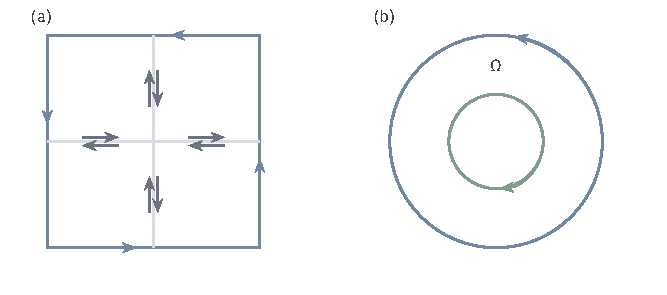
\includegraphics[width=112mm]{figures/01-mathematical-preliminaries-upper/01-mathematical-language-combinatorics-analysis-optimization/tikz/chapter3-concept-processes/boundary-orientation-cancellation.pdf}
 \caption{(a) 四个小正方形各取逆时针正向，共同边被沿相反方向走过；灰箭头略错开以便辨认，实际是同一条边。相加后只留下蓝色外边界。(b) 圆环的外边界逆时针、孔洞边界顺时针，沿任一边界前进时区域均在左侧。曲面拼片时也按公共边相反方向保证Stokes边界项相消。}
 \label{fig:analysis-process-boundary-orientation-cancellation}
\end{figure}

\subsection{平面区域积分与边界路径积分}

在平面上，区域的边界是一维路径。对同一个二维向量场，可以沿边界累计切向分量，得到环流；也可以累计外法向分量，得到通量。
两种边界积分分别对应区域内部的$Q_x-P_y$和散度$P_x+Q_y$。

\subsubsection{Green公式的环流形式}

旋度一节在小正方形上算出：逆时针环流约等于$Q_x-P_y$乘正方形面积。
把区域$\Omega$划分成许多小正方形（靠近弯曲边界处是不规则的小块），对每块写出这一近似再相加。
相邻两块的公共边在两块中方向相反，贡献抵消，剩下的只有沿$\Omega$正向边界的环流；另一侧各块“$Q_x-P_y$乘面积”之和，则是区域积分的近似和。
Green公式说明，在适当条件下这一近似在加细后成为精确等式：区域内各处微小旋转的累计，等于沿边界走一圈的总环流。
\begin{theorem}[Green公式]
\label{thm:multivariable-green}
设$\Omega\subseteq\mathbb R^2$为有界开区域，边界由有限条分段$C^1$简单闭曲线组成，
且区域在每段光滑边界附近位于边界的一侧。边界取正向，即外边界逆时针、孔洞边界顺时针。
若二维向量场$\bm F=(P,Q)^\top$在$\overline\Omega$的开邻域内连续可微，则\term{Green公式}（Green's theorem）给出
\begin{equation}
 \oint_{\partial\Omega}P\,\mathrm dx+Q\,\mathrm dy
 =\iint_\Omega\left(\frac{\partial Q}{\partial x}-\frac{\partial P}{\partial y}\right)\,\mathrm dx\,\mathrm dy.
 \label{eq:multivariable-green}
\end{equation}
\end{theorem}
左侧是向量场的切向路径积分；右侧是标量函数$Q_x-P_y$的区域积分。
在矩形上，二者的等式可以直接由一元基本定理和Fubini定理推出。
\begin{proof}[矩形情形的证明]
取$\Omega=(a,b)\times(c,d)$，先写出左侧沿四条边的贡献。下边$(t,c)$、$a\leq t\leq b$从左向右，$\mathrm dy=0$，贡献$\int_a^bP(x,c)\,\mathrm dx$；
上边从$(b,d)$走到$(a,d)$，贡献$-\int_a^bP(x,d)\,\mathrm dx$；右边从下向上，贡献$\int_c^dQ(b,y)\,\mathrm dy$；左边从上向下，贡献$-\int_c^dQ(a,y)\,\mathrm dy$。
水平边上$\mathrm dy=0$，竖直边上$\mathrm dx=0$，所以$Q$只在竖直边出现，$P$只在水平边出现。

再看右侧。场在闭矩形附近连续可微，以下被积函数均可积。固定$x$，对$y$用一元基本定理得$\int_c^d\partial_yP(x,y)\,\mathrm dy=P(x,d)-P(x,c)$；再对$x$积分，并由Fubini定理换成区域积分。对$Q$则先固定$y$、对$x$积分。于是
\[
 \begin{aligned}
 -\iint_\Omega\partial_yP\,\mathrm dx\,\mathrm dy
 &=\int_a^b[P(x,c)-P(x,d)]\,\mathrm dx,\\
 \iint_\Omega\partial_xQ\,\mathrm dx\,\mathrm dy
 &=\int_c^d[Q(b,y)-Q(a,y)]\,\mathrm dy.
 \end{aligned}
\]
第一行恰是下边与上边的两项，第二行恰是右边与左边的两项。
四项合起来，正是沿下、右、上、左四条边逆时针行进得到的路径积分。
\end{proof}
有限个矩形拼接时，公共边上的积分因方向相反而抵消。
一般规则区域的证明还需处理区域分片及边界逼近误差，不能仅凭小矩形上的等式完成；这里引用一般形式，完整论证可参考向量微积分教材\scite{math-strang1991calculus}。

先用旋转场在单位圆盘上核对公式两侧，并观察边界方向的作用。
\begin{example}[旋转场在单位圆盘上的Green公式]
\label{ex:analysis-rotation-field-green-disk}
取$\bm F=(P,Q)^\top=(-y,x)^\top$，$\Omega$为单位圆盘。$\bm F$在整个平面上连续可微，定理条件满足。
右侧被积函数为$Q_x-P_y=1-(-1)=2$，区域积分为$2\cdot\pi=2\pi$。
左侧取逆时针边界$\gamma(t)=(\cos t,\sin t)^\top$，$0\leq t\leq2\pi$，则$\bm F(\gamma(t))^\top\gamma'(t)=\sin^2t+\cos^2t=1$，积分同样为$2\pi$。
若把圆周改为顺时针，左侧变为$-2\pi$，右侧仍为$2\pi$，等式不再成立。
\end{example}
区域积分不含方向信息，边界积分却随方向反转而变号；Green公式的符号由正向边界的约定决定。

Green公式也可以反过来使用：选一个满足$Q_x-P_y\equiv1$的场，右侧就是区域的面积，于是面积可以由边界环流算出。
\begin{example}[用边界计算面积]
\label{ex:analysis-green-area-formula}
设$\Omega$满足定理~\ref{thm:multivariable-green}的条件。取$P=-y/2$、$Q=x/2$，则$Q_x-P_y=1$，Green公式给出
\[
 \operatorname{area}(\Omega)=\frac12\oint_{\partial\Omega}x\,\mathrm dy-y\,\mathrm dx.
\]
对半轴为$\alpha,\beta>0$的椭圆区域，正向边界取$\gamma(t)=(\alpha\cos t,\beta\sin t)^\top$、$0\leq t\leq2\pi$。这时$\mathrm dx=-\alpha\sin t\,\mathrm dt$、$\mathrm dy=\beta\cos t\,\mathrm dt$，
\[
 x\,\mathrm dy-y\,\mathrm dx=(\alpha\beta\cos^2t+\alpha\beta\sin^2t)\,\mathrm dt=\alpha\beta\,\mathrm dt,
\]
所以面积为$\frac12\cdot2\pi\alpha\beta=\pi\alpha\beta$。
\end{example}
这个公式只需要沿边界走一圈、记录坐标与位移，就能得到所围面积；机械求积仪正是按这一原理工作的。

定理要求场在$\overline\Omega$的开邻域内连续可微。区域包含场的奇点时，这一条件不再满足，下面的例子说明它不能省略。
\begin{example}[有孔区域上的涡旋场]
\label{ex:analysis-annulus-vortex-green}
第~\ref{sec:multivariable-potential-path-independence}节的穿孔平面反例中，$\bm F=(-y,x)^\top/(x^2+y^2)$在原点以外满足$Q_x-P_y=0$，但沿单位圆逆时针一周的环流为$2\pi$。

取圆环$\Omega=\{1<x^2+y^2<4\}$。它的闭包不含原点，$\bm F$在$\overline\Omega$的一个开邻域内连续可微，Green公式适用，右侧为$0$。
左侧由两圈组成。外圈$r=2$逆时针，参数化为$(2\cos t,2\sin t)^\top$，此时$\bm F=(-\sin t,\cos t)^\top/2$，与速度$(-2\sin t,2\cos t)^\top$的内积为$1$，环流为$2\pi$；内圈$r=1$按正向取顺时针，环流为$-2\pi$。两者相加为零，与右侧一致。
\end{example}
外圈逆时针为$2\pi$、内圈顺时针为$-2\pi$，也就是说，两条圆周按同一逆时针方向走时环流都是$2\pi$。环流来自场在原点处的奇异，而不是来自圆环内部。
单位圆盘含有原点，$\bm F$在那里无定义，不满足Green公式的条件，所以不能由$Q_x-P_y=0$推出单位圆上的环流为零。

\subsubsection{Green公式的通量形式}

现在把平面向量场想成薄层流体的速度场，问单位时间有多少流体穿过区域边界流出。
每个小正方形的净流出约等于散度乘面积；相邻两块的公共边上外法向相反，一块的流出就是另一块的流入，相加后抵消。
因此可以预期：区域内部源强度的总和，等于穿过边界的净流出。

计算通量需要把场投影到外法向上。正向边界的有向位移是$\bm\tau\,\mathrm ds=(\mathrm dx,\mathrm dy)^\top$，而外法向由$\bm\tau$顺时针转过直角得到，因此
\[
 \bm n\,\mathrm ds=(\mathrm dy,-\mathrm dx)^\top.
\]
这一关系把法向通量写成切向路径积分，从而可以使用Green公式。
\begin{theorem}[平面区域的通量公式]
\label{thm:multivariable-planar-flux}
在与Green公式相同的区域条件下，若$\bm F=(F_1,F_2)^\top$在$\overline\Omega$的开邻域内连续可微，
$\bm n$是边界的外单位法向，则
\[
 \int_{\partial\Omega}\bm F^\top\bm n\,\mathrm ds
 =\iint_\Omega\operatorname{div}\bm F\,\mathrm dx\,\mathrm dy.
\]
\end{theorem}
\begin{proof}
利用外法向与正向边界的关系，$\bm F^\top\bm n\,\mathrm ds=F_1\,\mathrm dy-F_2\,\mathrm dx$，所以左侧等于
$\oint_{\partial\Omega}(-F_2)\,\mathrm dx+F_1\,\mathrm dy$。
在Green公式中取$(P,Q)=(-F_2,F_1)$，右侧被积函数为$Q_x-P_y=\partial_xF_1+\partial_yF_2=\operatorname{div}\bm F$。
\end{proof}
这也是二维的散度公式。它与环流形式使用相同的区域条件，但累计的边界分量和内部导数不同。

下面在单位圆盘上比较两个场的通量：一个从各处均匀发散，一个只绕原点打转。
\begin{example}[单位圆盘上径向场与旋转场的通量]
取$\bm F(x,y)=(x,y)^\top$，$\Omega$为单位圆盘。散度为$1+1=2$，区域积分为$2\pi$。
边界参数化为$\gamma(t)=(\cos t,\sin t)^\top$，$0\leq t\leq2\pi$，外法向$\bm n=\gamma(t)$，$\mathrm ds=\mathrm dt$，且$\bm F^\top\bm n=\cos^2t+\sin^2t=1$，所以边界通量也为$2\pi$。若改取内法向，通量变为$-2\pi$。

再取旋转场$\bm G=(-y,x)^\top$。它的散度为$0+0=0$；在单位圆上$\bm G^\top\bm n=-y\cdot x+x\cdot y=0$，通量为零，两侧一致。它的环流却是示例~\ref{ex:analysis-rotation-field-green-disk}算出的$2\pi$。
\end{example}
径向场好比流体在圆盘内各处均匀产生，产生的总量全部从圆周流出。旋转场则像杯中被搅动的水：水在杯中打转，却没有流出杯壁。通量与环流记录的是边界上两个不同的分量。

\subsection{空间区域积分与边界曲面积分}

将平面区域换成三维空间区域后，边界从曲线变成闭曲面。
对应关系仍然是内部散度的积分等于边界净通量；由这一关系还可以推出多元函数的分部积分公式。

\subsubsection{Gauss公式}

仍把$\bm F$看作流体的速度场。区域$\Omega$内各处的散度给出单位体积的产生率，其体积积分是单位时间在$\Omega$内产生的流体总量。
流体总量守恒时，新产生的流体只能穿过边界离开，所以这个总量应等于穿过$\partial\Omega$的外向净通量。
从计算上看，把$\Omega$切成小立方体，每块的净流出约等于散度乘体积；相邻两块的公共面上外法向相反，流出与流入相消，只留下外边界上的通量。
静电学中有同样的关系：电场穿过闭曲面的通量，由闭曲面内的总电荷决定\scite{math-openstax-calculus3}。
Gauss散度定理给出这一平衡精确成立的条件。
\begin{theorem}[Gauss散度定理]
\label{thm:analysis-divergence-theorem}
设$\Omega\subseteq\mathbb R^3$为有界开区域，其边界是由有限个正则$C^1$曲面片组成的闭曲面。
各片内部互不相交，接缝为有限条分段$C^1$曲线及有限个点；在每个光滑边界点附近，区域位于边界的一侧。
若向量场$\bm F$在$\overline\Omega$的一个开邻域内连续可微，则\term{散度定理}（divergence theorem）给出
\begin{equation}
  \int_{\Omega}\nabla\mathbin{\cdot}\bm F\,\mathrm d\bm x
  =\int_{\partial\Omega}\bm F^\top\bm n\,\mathrm dS,
 \label{eq:analysis-divergence-theorem}
\end{equation}
其中$\bm n$是光滑边界片上的外单位法向，$\mathrm dS$为面积元素。
\end{theorem}
光滑有界区域和通常的多面体满足这些条件。接缝的曲面面积为零，不影响通量积分；$\bm F$及其偏导数在紧集$\overline\Omega$上连续因而有界，所以两侧积分都有限。
左侧累计向量场的局部净流出率，右侧累计穿过整个外边界的净通量。

对长方体，这一等式不需要借助一般曲面逼近，可以逐坐标证明；证明正是把散度一节中小立方体上的近似计算改写成精确等式。
\begin{proof}[长方体情形的证明]
取$\Omega=(a,b)\times(c,d)\times(e,f)$。
固定$(y,z)$，对$x$用一元基本定理，再由Fubini定理对$(y,z)$积分，得到
\[
 \int_\Omega\partial_xF_1\,\mathrm d\bm x
 =\int_c^d\int_e^f
   [F_1(b,y,z)-F_1(a,y,z)]\,\mathrm dz\,\mathrm dy.
\]
在$x=b$面上外法向为$(1,0,0)^\top$，$\bm F^\top\bm n=F_1$；在$x=a$面上外法向为$(-1,0,0)^\top$，$\bm F^\top\bm n=-F_1$。所以右侧正是这两张面的外向通量之和。
同样，$\partial_yF_2$的体积积分等于$y=d$与$y=c$两面的通量之和，
$\partial_zF_3$的体积积分等于$z=f$与$z=e$两面的通量之和。在其余各面上，相应分量与法向垂直，不贡献这一项。
三式相加，左侧为散度的体积积分，右侧为六张面的全部外向通量。
\end{proof}
拼接长方体时，公共面上的外法向相反，内部通量恰好抵消。
从长方体推广到定理中的一般规则区域，还需对边界分片和逼近作严格处理；一般形式在这里引用，证明可参考向量微积分教材\scite{math-strang1991calculus}。
无界区域、弱导数或更不规则的边界，需要另用相应版本，不能由长方体情形直接推出。


图~\ref{fig:analysis-process-gauss-shared-face}显示体积小块相加时，共同面上的两份通量为什么消失。
\begin{figure}[!htbp]
 \centering
 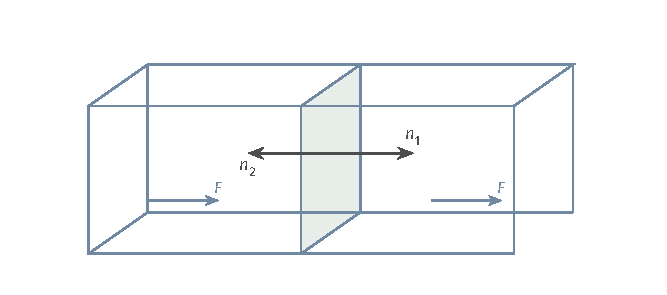
\includegraphics[width=112mm]{figures/01-mathematical-preliminaries-upper/01-mathematical-language-combinatorics-analysis-optimization/tikz/chapter3-concept-processes/gauss-shared-face.pdf}
 \caption{两个相邻单位立方体共用绿色面，图用斜投影表示三维几何。取常场$F=(1,0,0)^\top$，共同面上两侧外法向为$n_1=(1,0,0)^\top$与$n_2=-n_1$，对应通量为$1,-1$，相加抵消。整体外向净通量也为零，与散度为零一致；一般区域的散度定理仍需要前述条件与证明。}
 \label{fig:analysis-process-gauss-shared-face}
\end{figure}

先用一个答案已知的计算核对散度定理。
\begin{example}[用散度定理核对球面面积]
设$B_R$是以原点为中心、半径$R>0$的球，边界球面取外法向。令$\bm F(\bm x)=\bm x/R$，它在整个$\mathbb R^3$上连续可微。
球面上$\bm n=\bm x/R=\bm F$，所以$\bm F^\top\bm n=1$，外向通量等于球面面积。
另一方面，$\operatorname{div}\bm F=3/R$，散度定理给出
\[
 \int_{\partial B_R}\bm F^\top\bm n\,\mathrm dS
 =\frac3R\operatorname{vol}(B_R)
 =\frac3R\cdot\frac{4\pi R^3}3=4\pi R^2.
\]
\end{example}
这里的球体积已在第~\ref{sec:multivariable-change-variables}节用球坐标算出；所得结果与第~\ref{sec:analysis-surface-integration}节直接参数化球面求得的面积一致。

定理要求$\bm F$在$\overline\Omega$的一个开邻域内连续可微。点源场在原点无定义，下面用它检查这一条件的作用。
\begin{example}[点源的通量]
\label{ex:analysis-point-source-flux}
在$\mathbb R^3\setminus\{\bm0\}$上取$\bm F(\bm x)=\bm x/\lVert\bm x\rVert_2^3$，记$r=\lVert\bm x\rVert_2$。由$\partial_jr=x_j/r$，
\[
 \partial_j\Bigl(\frac{x_j}{r^3}\Bigr)=\frac1{r^3}-\frac{3x_j^2}{r^5},
 \qquad
 \operatorname{div}\bm F=\frac3{r^3}-\frac{3r^2}{r^5}=0.
\]
但在半径为$R$的球面上，外法向为$\bm x/R$，$\bm F^\top\bm n=1/R^2$，外向通量为$4\pi R^2/R^2=4\pi$。
这并不与散度定理矛盾：球体含有原点，而$\bm F$在原点无定义，定理的条件不满足。

对不含原点的球壳$R_1<r<R_2$，定理适用，左侧为零。外球面的外向通量为$4\pi$；内球面的外法向指向原点，通量为$-4\pi$；两者相加确为零。
\end{example}
所以以原点为中心的球面上的通量都是$4\pi$，与半径无关：场在原点以外处处无源，全部通量都来自原点处的点源。
静电学中，位于原点的点电荷$q$产生的电场是$\frac{q}{4\pi\varepsilon_0}\bm F$，其中$\varepsilon_0$为真空介电常数；它穿过以原点为中心的球面的通量为$q/\varepsilon_0$，这就是Gauss定律在点电荷上的形式。

\paragraph{散度是通量密度}

已证明的长方体情形，足以把散度一节的近似推导变成精确结论。
设$\bm F$在开集$U$上连续可微，$\bm a\in U$，$Q_h$是以$\bm a$为中心、边长为$h$的立方体；$h$足够小时$\overline{Q_h}\subseteq U$。由长方体上的Gauss公式，
\[
 \frac1{h^3}\int_{\partial Q_h}\bm F^\top\bm n\,\mathrm dS
 =\frac1{h^3}\int_{Q_h}\operatorname{div}\bm F\,\mathrm d\bm x.
\]
右侧是散度在$Q_h$上的平均值，它与$\operatorname{div}\bm F(\bm a)$的差不超过$\sup_{Q_h}|\operatorname{div}\bm F-\operatorname{div}\bm F(\bm a)|$。散度连续，所以$h\to0$时这个上界趋于零，平均值趋于$\operatorname{div}\bm F(\bm a)$。

这说明散度确实是“单位体积的净流出”的极限。把立方体换成以$\bm a$为中心的小球，用一般的Gauss公式可以得到同样的极限。小球的取法不依赖坐标轴，所以散度描述的是场本身的性质，不依赖坐标系的方向。

\subsubsection{多元分部积分}

一元分部积分（式~\eqref{eq:analysis-integration-by-parts}）把一个因子的导数转给另一个因子，并留下端点项。设$u$在$[a,b]$上连续可微、$v$二阶连续可微，把式中的$v$换成$v'$，得到
\[
 \int_a^bu\,v''\,\mathrm dx
 =u(b)v'(b)\cdot(+1)+u(a)v'(a)\cdot(-1)-\int_a^bu'v'\,\mathrm dx.
\]
这里把端点项$[uv']_a^b$拆开写：区间在右端点的外法向是$+1$，在左端点是$-1$。

推广到多元情形时，各项依次对应：二阶导数$v''$换成$\Delta v$，一阶导数的乘积$u'v'$换成梯度的内积$\nabla u^\top\nabla v$，两个端点换成边界曲面，“$v'$乘外法向$\pm1$”换成$\nabla v^\top\bm n$，即$v$沿外法向的方向导数。
对乘积向量场$u\nabla v$使用散度定理，就得到这一推广。
\begin{theorem}[多元分部积分]
\label{thm:multivariable-integration-by-parts}
设$\Omega\subseteq\mathbb R^3$满足上述Gauss公式的区域条件。
若标量函数$u$在$\overline\Omega$的开邻域内连续可微，$v$在同一邻域内二阶连续可微，则
\[
 \int_\Omega u\Delta v\,\mathrm d\bm x
 =\int_{\partial\Omega}u\nabla v^\top\bm n\,\mathrm dS
  -\int_\Omega\nabla u^\top\nabla v\,\mathrm d\bm x.
\]
\end{theorem}
\begin{proof}
向量场$\bm F=u\nabla v$的第$j$个分量是$u\,\partial_jv$，它连续可微。由一元乘积法则，
$\partial_j(u\,\partial_jv)=\partial_ju\,\partial_jv+u\,\partial_j^2v$，对$j$求和得到
\[
 \operatorname{div}(u\nabla v)
 =\nabla u^\top\nabla v+u\Delta v.
\]
将它代入Gauss公式，再把$\nabla u^\top\nabla v$的区域积分移到等式另一侧，即得结论。
\end{proof}
对满足Green公式条件的平面区域，同样的证明改用平面通量公式（定理~\ref{thm:multivariable-planar-flux}）即可，边界面积元素相应换成弧长元素。
这一公式把$v$的二阶导数转移为$u$与$v$的一阶导数，同时保留法向边界项；该项是否为零，必须由具体边界条件决定。

取$u=1$，公式化为$\int_\Omega\Delta v\,\mathrm d\bm x=\int_{\partial\Omega}\nabla v^\top\bm n\,\mathrm dS$，也就是对梯度场$\nabla v$使用散度定理。下面在球上核对这一特例。
\begin{example}[球上平方范数的Laplace积分]
取以原点为中心、半径为$R$的球$B_R$和$v(\bm x)=\lVert\bm x\rVert_2^2$。
左侧：$\Delta v=6$，所以$\int_{B_R}\Delta v\,\mathrm d\bm x=6\operatorname{vol}(B_R)=6\cdot\frac{4\pi R^3}3=8\pi R^3$。
右侧：球面上$\nabla v=2\bm x$，外法向$\bm n=\bm x/R$，故$\nabla v^\top\bm n=2\lVert\bm x\rVert_2^2/R=2R$，积分为$2R\cdot4\pi R^2=8\pi R^3$。两侧相等。
\end{example}

边界项为零时，公式可以给出结构性的结论。下面用它说明Laplace方程的解由边界值唯一确定。
\begin{example}[Laplace方程的解由边界值决定]
设$\Omega$满足Gauss公式的区域条件，$w$在$\overline\Omega$的开邻域内二阶连续可微，在$\Omega$内$\Delta w=0$，在$\partial\Omega$上$w=0$。
在定理~\ref{thm:multivariable-integration-by-parts}中取$u=v=w$。左侧被积函数$w\Delta w$为零；边界项的被积函数含因子$w$，也为零。于是
\[
 \int_\Omega\lVert\nabla w\rVert_2^2\,\mathrm d\bm x=0.
\]
被积函数连续且非负；若它在某点为正，则在该点的一个邻域内为正，积分也为正。所以在开集$\Omega$上$\nabla w$恒为零。
$\Omega$是连通的开区域，所以$w$在$\Omega$上为常数；再由$w$在$\overline\Omega$上连续且在边界上为零，得$w\equiv0$。

现在设$v_1,v_2$都在$\overline\Omega$的开邻域内二阶连续可微，在$\Omega$内满足$\Delta v_1=\Delta v_2=0$，在$\partial\Omega$上取值相同。差$w=v_1-v_2$满足上面的全部条件，所以$v_1=v_2$。
\end{example}
按热传导的解释，稳定的温度分布由边界温度唯一决定。

\subsection{曲面积分与边界路径积分}

Gauss公式要求闭曲面围成空间区域。另一类问题只给一张有边界的定向曲面，要求比较曲面上的旋转累计与边界环流。
这时使用旋度在曲面法向上的分量，不需要先把曲面补成闭曲面。

\subsubsection{Stokes公式}

在$z=0$平面上取向上法向时，旋度的法向分量$(\nabla\times\bm F)^\top\bm e_3$就是Green公式中的$Q_x-P_y$。
对空间中的弯曲曲面，可以把它切成许多很小的曲面片，每片近似是一小块平面。在法向为$\bm n$的小平面片上，边界环流约等于$(\nabla\times\bm F)^\top\bm n$乘面积。
各片采用相容定向时，相邻两片的公共边被沿相反方向走过，环流相消，只剩整张曲面的边界。
用桨轮的图像说：在曲面上各处放置转轴沿法向的小桨轮，它们感受到的旋转强度按面积累加，总和等于沿曲面边缘走一圈的环流。
Stokes公式把这一关系写成精确等式，同时要求法向与边界方向相容。
\begin{theorem}[Stokes定理]
\label{thm:multivariable-stokes}
设$S\subseteq\mathbb R^3$为紧致、可定向的分片$C^2$曲面，边界由有限条分段$C^1$简单闭曲线组成。
各光滑曲面片选取连续且片间定向相容的单位法向$\bm n$，边界采用其诱导方向。
若向量场$\bm F$在$S$的开邻域内连续可微，则\term{Stokes公式}（Stokes' theorem）给出
\begin{equation}
 \oint_{\partial S}\bm F^\top\,\mathrm d\bm r
 =\int_S(\nabla\times\bm F)^\top\bm n\,\mathrm dS.
 \label{eq:multivariable-stokes}
\end{equation}
\end{theorem}
这里的“可定向”要求各曲面片能相容地选择法向，使公共边上的诱导方向相反；有折角的接缝处不要求存在唯一法向。
两侧都为标量：左侧是原向量场的边界环流，右侧是其旋度穿过曲面的通量。

在一张参数曲面片上，可以把公式归结为参数平面上的Green公式。
设参数域$D$满足Green公式的区域条件，$\bm r(u,v)$在$D$的邻域内二阶连续可微、在内部正则且一一对应，并采用$\bm r_u\times\bm r_v$确定的定向。
还要求$\partial D$的正向经$\bm r$对应曲面片边界的诱导方向，从而可以把边界路径积分放到$\partial D$上计算。
这里的$u,v$是参数，与多元分部积分中的函数$u,v$无关。记
\[
 \begin{aligned}
 A(u,v)&=\bm F(\bm r(u,v))^\top\bm r_u(u,v),\\
 B(u,v)&=\bm F(\bm r(u,v))^\top\bm r_v(u,v).
 \end{aligned}
\]

先处理左侧。若$(u(t),v(t))$沿$\partial D$行进，曲面边界上对应的点是$\bm r(u(t),v(t))$，由链式法则，其速度为$\bm r_uu'(t)+\bm r_vv'(t)$。
与$\bm F$取内积，得$\bm F^\top\mathrm d\bm r=A\,\mathrm du+B\,\mathrm dv$，所以左侧等于参数平面上的路径积分$\oint_{\partial D}A\,\mathrm du+B\,\mathrm dv$。

再计算参数平面上Green公式右侧的被积函数$\partial_uB-\partial_vA$。记$\bm J_{\bm F}$为$\bm F$的Jacobian矩阵，其元素为$(\bm J_{\bm F})_{i,j}=\partial_jF_i$。由链式法则和乘积法则，
\[
 \begin{aligned}
 \partial_uB&=(\bm J_{\bm F}\bm r_u)^\top\bm r_v+\bm F^\top\bm r_{vu},\\
 \partial_vA&=(\bm J_{\bm F}\bm r_v)^\top\bm r_u+\bm F^\top\bm r_{uv},
 \end{aligned}
\]
其中$\bm J_{\bm F}$与$\bm F$在$\bm r(u,v)$处取值。$\bm r$二阶连续可微，混合偏导相等，$\bm r_{uv}=\bm r_{vu}$，所以两式相减时含二阶导数的项抵消。
又$(\bm J_{\bm F}\bm r_u)^\top\bm r_v=\bm r_v^\top\bm J_{\bm F}\bm r_u$、$(\bm J_{\bm F}\bm r_v)^\top\bm r_u=\bm r_v^\top\bm J_{\bm F}^\top\bm r_u$，于是
\[
 \partial_uB-\partial_vA=\bm r_v^\top(\bm J_{\bm F}-\bm J_{\bm F}^\top)\bm r_u.
\]

接下来把右端写成旋度。反对称矩阵$\bm W=\bm J_{\bm F}-\bm J_{\bm F}^\top$的元素为$\bm W_{i,j}=\partial_jF_i-\partial_iF_j$；逐个分量对照旋度的定义可以验证，对任意$\bm a\in\mathbb R^3$都有$\bm W\bm a=(\nabla\times\bm F)\times\bm a$。
再用混合积的轮换关系$\bm b^\top(\bm c\times\bm a)=\bm c^\top(\bm a\times\bm b)$（两边都等于以$\bm a,\bm b,\bm c$为列的行列式），取$\bm a=\bm r_u$、$\bm b=\bm r_v$、$\bm c=\nabla\times\bm F$，得到
\[
 \partial_uB-\partial_vA
 =\bigl(\operatorname{curl}\bm F\bigr)(\bm r(u,v))^\top
   (\bm r_u\times\bm r_v).
\]
右端乘$\mathrm du\,\mathrm dv$，正是曲面通量积分（式~\eqref{eq:analysis-surface-flux}）中的被积项。

$A,B$由连续可微的$\bm F$与二阶连续可微的$\bm r$及其一阶导数复合、相乘而成，在$D$的邻域内连续可微，所以参数平面上的Green公式适用；它给出该曲面片上的Stokes公式。
对有限张相容定向的曲面片，公共边的路径积分相消，只剩整张曲面的边界。
一般分片曲面的完整论证还需核对曲面覆盖及接缝条件；以上推导只说明参数片上的机制，一般定理可参考向量微积分教材\scite{math-strang1991calculus}。

\paragraph{旋度分量是环流密度}

Stokes公式也给出旋度含义的精确形式。设$\bm F$在$\bm a$附近连续可微，$\bm n$是单位向量，$D_\rho$是以$\bm a$为圆心、半径为$\rho$、垂直于$\bm n$并取法向$\bm n$的平面圆盘。由Stokes公式，
\[
 \frac1{\pi\rho^2}\oint_{\partial D_\rho}\bm F^\top\,\mathrm d\bm r
 =\frac1{\pi\rho^2}\int_{D_\rho}(\nabla\times\bm F)^\top\bm n\,\mathrm dS,
\]
右侧是$(\nabla\times\bm F)^\top\bm n$在圆盘上的平均值。旋度连续，所以$\rho\to0$时它趋于$(\nabla\times\bm F)(\bm a)^\top\bm n$。
因此，旋度沿$\bm n$的分量就是垂直于$\bm n$的微小圆周上的环流除以所围面积的极限。这正是桨轮图像所描述的量；圆盘的取法不依赖坐标轴，所以这一含义也不依赖坐标轴的选取。

\subsubsection{跨接曲面的选择}

Stokes公式的左侧只由有向边界和边界上的向量场决定。因此，若两张满足定理条件的定向曲面具有同一有向边界，
且$\bm F$在两张曲面附近都连续可微，则两张曲面上的旋度通量相等。
计算时可以选较简单的跨接曲面，但必须核对向量场定义域，不能让替换曲面穿过场的奇点。

这一结论也可以从Gauss公式得到印证。若$\bm F$二阶连续可微，则
\[
 \operatorname{div}(\nabla\times\bm F)
 =\partial_x(\partial_yF_3-\partial_zF_2)
 +\partial_y(\partial_zF_1-\partial_xF_3)
 +\partial_z(\partial_xF_2-\partial_yF_1)=0,
\]
最后的等号成立，是因为混合偏导相等，六项两两抵消。设两张跨接曲面恰好围成一个满足Gauss公式条件的区域，且$\bm F$在该区域闭包的开邻域内二阶连续可微。
区域的外法向在一张曲面上与所选法向相同，在另一张上相反；旋度场的散度为零，所以散度定理说明两张曲面上的旋度通量之差为零。

下面用同一个场在单位圆上比较两张跨接曲面。
\begin{example}[单位圆上的圆盘与半球面]
取$\bm F=(-y/2,x/2,0)^\top$，它在整个$\mathbb R^3$上连续可微，示例~\ref{ex:analysis-rigid-rotation-curl}已算出$\nabla\times\bm F=(0,0,1)^\top$。单位圆$\{x^2+y^2=1,\ z=0\}$采用从上方看逆时针的方向。

先取向上单位圆盘$S_1$。由示例~\ref{ex:analysis-hemisphere-induced-orientation}，它的诱导方向正是这一方向；旋度的法向分量为$1$，所以
\[
 \oint_{\partial S_1}\bm F^\top\,\mathrm d\bm r
 =\iint_{S_1}1\,\mathrm dS=\pi.
\]
直接计算左侧也得到同一结果：取$\gamma(t)=(\cos t,\sin t,0)^\top$，$0\leq t\leq2\pi$，则$\bm F(\gamma(t))^\top\gamma'(t)=\tfrac12(\sin^2t+\cos^2t)=\tfrac12$，积分为$\pi$。

再取外向上半单位球面$S_2$，同一例子说明它的诱导方向与$S_1$相同。用第~\ref{sec:analysis-surface-integration}节的球面参数$(\varphi,\theta)$，$0\leq\varphi\leq\pi/2$，外法向为$\bm n=\bm x$，旋度的法向分量为$z=\cos\varphi$，面积元为$\sin\varphi\,\mathrm d\varphi\,\mathrm d\theta$，所以
\[
 \int_{S_2}(\nabla\times\bm F)^\top\bm n\,\mathrm dS
 =\int_0^{2\pi}\int_0^{\pi/2}\cos\varphi\sin\varphi\,\mathrm d\varphi\,\mathrm d\theta
 =2\pi\cdot\frac12=\pi,
\]
与圆盘上的结果相同。
\end{example}
若改用向下定向的圆盘，边界方向也必须反转，两个积分同时变号。


图~\ref{fig:analysis-process-stokes-spanning-surfaces}比较同一有向圆周的两张跨接曲面。替换曲面时，边界方向与场的定义域都要同时保留。
\begin{figure*}[!htbp]
 \centering
 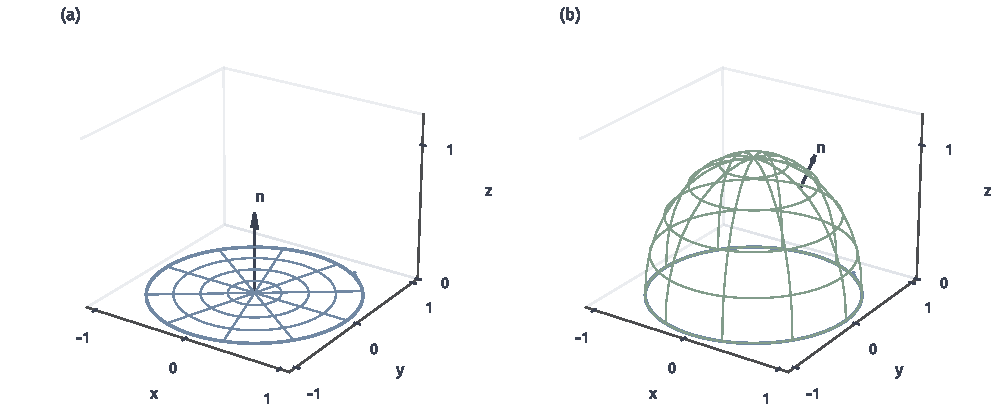
\includegraphics[width=169.0mm]{figures/01-mathematical-preliminaries-upper/01-mathematical-language-combinatorics-analysis-optimization/matplotlib/chapter3-concept-processes/stokes-spanning-surfaces.pdf}
 \caption{(a) 向上单位圆盘；(b) 外向上半单位球面。蓝色边界均从上方看逆时针，黑箭头标记各自法向。对$F=(-y/2,x/2,0)^\top$，旋度恒为$(0,0,1)^\top$，两面上的旋度通量都为$\pi$。右面面积为$2\pi$而非$\pi$；相等的是法向分量的累计，不能把通量当成面积。}
 \label{fig:analysis-process-stokes-spanning-surfaces}
\end{figure*}

\subsection{积分公式的比较}

本节各公式回答的都是同一类问题：导数在内部的积分与边界积分之间的关系。推导方式也相同：在小块上建立局部关系，再利用相容方向让内部边界相消。
它们的内部对象、边界对象和方向条件则各不相同。下表把一元基本定理与路径积分基本定理也列在一起，二者以区间或路径的两个端点为边界。
\begin{center}
\begin{tabular}{lll}
\toprule
公式 & 内部积分 & 边界积分\\
\midrule
一元基本定理 & 区间上的$f'$ & 端点值之差$f(b)-f(a)$\\
路径积分基本定理 & 路径上$\nabla\phi$的切向积分 & 端点值之差\\
Green环流形式 & 平面区域的$Q_x-P_y$ & 正向路径的切向积分\\
Gauss & 空间区域的散度 & 闭曲面的外向通量\\
Stokes & 定向曲面的旋度通量 & 诱导方向的路径环流\\
\bottomrule
\end{tabular}
\end{center}
对向上定向的平面曲面，Stokes公式还原为Green公式的环流形式；Green公式的通量形式则是二维的散度公式。
普通标量函数的区域积分不自动具有边界表达：要使用这些公式，须先找到满足条件的向量场，使其散度或旋度的相应分量等于被积函数。示例~\ref{ex:analysis-green-area-formula}的面积公式就是先选出满足$Q_x-P_y\equiv1$的场。

Stokes公式还解释了第~\ref{sec:multivariable-potential-path-independence}节中势函数的存在为何与定义域有关。设$\bm F$在开集$U\subseteq\mathbb R^3$上连续可微且$\nabla\times\bm F=\bm0$。若一条闭路径是$U$内某张满足定理条件的定向曲面的有向边界，则该闭路径上的环流等于旋度的通量，也就是零。
在星形域中，闭路径上各点与中心点之间的线段扫出一张锥面，它整个落在定义域内，不会碰到场的奇点；这与那里在星形域上构造势函数的结论一致。
穿孔平面上绕原点的单位圆则不同：在平面内，以它为边界的区域只能是单位圆盘，必然包含原点，而场在原点无定义；所以局部条件$Q_x-P_y=0$并不排除$2\pi$的环流（示例~\ref{ex:analysis-annulus-vortex-green}）。

各公式均使用勒贝格积分。连续可微性、分片规则边界与定向是这里的经典公式所需的条件，并不是另换一种积分定义。
尤其要核对向量场是否在整个积分对象附近都有定义：穿孔平面上的涡旋场在原点无定义，不能把包含原点的圆盘直接代入Green公式；点源场也不能直接用于包含原点的球体（示例~\ref{ex:analysis-point-source-flux}）。
区域积分不能区分只在零测集上不同的函数，而本节区域的边界由有限条曲线或有限个曲面片组成，在相应的面积或体积测度下正是零测集；所以仅知道两个函数在区域上几乎处处相等，不足以确定它们的边界积分。
如果要降低导数或边界的规则性，还须另外建立弱导数、边界迹及相应的积分公式；不能沿用当前公式而省去这些条件。

\FloatBarrier
